\documentclass[10pt,twocolumn]{article}

\usepackage[letterpaper,margin=0.56in]{geometry}
\usepackage{amsmath,amssymb,graphicx,booktabs,threeparttable,natbib,float,subcaption,placeins}
\usepackage[T1]{fontenc}
\usepackage[utf8]{inputenc}
\usepackage{lmodern}
\usepackage{caption}
\usepackage{hyperref}
\hypersetup{colorlinks=true, linkcolor=black, citecolor=blue, urlcolor=black}
\bibliographystyle{plainnat}
\setcitestyle{authoryear,round}
\captionsetup{font=scriptsize,labelfont=bf}
\captionsetup[subfigure]{font=scriptsize,skip=1pt}
\setlength{\floatsep}{4pt plus 1pt minus 1pt}
\setlength{\textfloatsep}{5pt plus 1pt minus 1pt}
\setlength{\dblfloatsep}{4pt plus 1pt minus 1pt}
\setlength{\dbltextfloatsep}{5pt plus 1pt minus 1pt}
\setcounter{topnumber}{4}
\setcounter{dbltopnumber}{4}
\renewcommand{\topfraction}{0.95}
\renewcommand{\dbltopfraction}{0.95}
\renewcommand{\textfraction}{0.03}
\renewcommand{\floatpagefraction}{0.85}
\renewcommand{\dblfloatpagefraction}{0.85}
\setlength{\parskip}{1pt}
\setlength{\parindent}{10pt}
\raggedbottom
\renewcommand{\abstractname}{Resumo}
\renewcommand{\refname}{Referências}
\renewcommand{\tablename}{Tabela}
\renewcommand{\figurename}{Figura}
\newcommand{\tabnotes}[1]{\par\vspace{2pt}\noindent\begin{minipage}{\linewidth}\footnotesize #1\end{minipage}}
\title{\vspace{-1.35cm}\textbf{Apêndice: robustez com pool RS}}
\author{Victor Rangel\textsuperscript{*}\\[-1pt]{\normalsize Insper}}
\date{}

\begin{document}
\maketitle

\section{Robustez com pool RS}

Este apêndice reporta a robustez dos quatro desfechos principais com pool restrito ao Rio Grande do Sul. Quando a rotina de Firpo e Possebom retorna conjunto vazio para a classe linear de efeitos, o painel de IC é deixado sem banda sombreada.

\begin{table}[H]
\centering
\caption{Robustez com pool RS}
\label{tab:appendix-results}
\begin{threeparttable}
\scriptsize
\begin{tabular}{l c r r r}
\toprule
Desfecho & Pool & Pós/pré & $p_{FP}$ & Efeito final \\
\midrule
Bolsa Família & RS & 5.54 & 0.062 & -320\textsuperscript{*} \\
Estoque formal & RS & 4.09 & 0.077 & 921\textsuperscript{*} \\
\bottomrule
\end{tabular}
\tabnotes{\textit{Notas:} A tabela reporta a robustez dos desfechos principais com pool restrito ao Rio Grande do Sul. Aplica-se o mesmo filtro de qualidade de ajuste pré-intervenção usado na tabela principal.}
\end{threeparttable}

\end{table}

\begin{figure*}[t]
\centering
\makebox[\textwidth][c]{%
\begin{minipage}{0.995\textwidth}
\centering
\subcaptionbox{Bolsa Família: Observado e sintético}[0.486\textwidth]{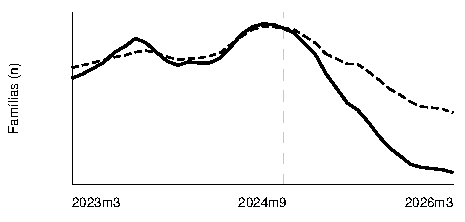
\includegraphics[width=0.486\textwidth]{figures/fig_app-rs_01_bolsa_familia_series.pdf}}\hspace{0.006\textwidth}%
\subcaptionbox{Estoque formal: Observado e sintético}[0.486\textwidth]{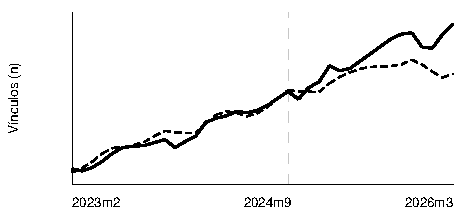
\includegraphics[width=0.486\textwidth]{figures/fig_app-rs_02_emprego_estoque_series.pdf}}

\vspace{2pt}
\subcaptionbox{Bolsa Família: Gap e IC 90\%}[0.486\textwidth]{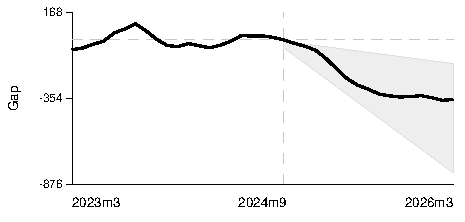
\includegraphics[width=0.486\textwidth]{figures/fig_app-rs_01_bolsa_familia_ci.pdf}}\hspace{0.006\textwidth}%
\subcaptionbox{Estoque formal: Gap e IC 90\%}[0.486\textwidth]{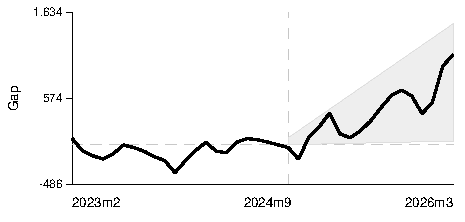
\includegraphics[width=0.486\textwidth]{figures/fig_app-rs_02_emprego_estoque_ci.pdf}}

\vspace{2pt}
\subcaptionbox{Bolsa Família: Placebos}[0.486\textwidth]{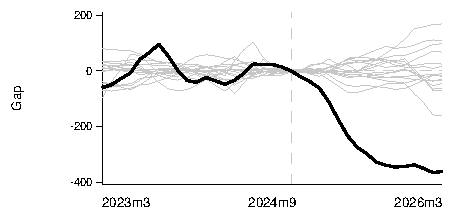
\includegraphics[width=0.486\textwidth]{figures/fig_app-rs_01_bolsa_familia_placebo.pdf}}\hspace{0.006\textwidth}%
\subcaptionbox{Estoque formal: Placebos}[0.486\textwidth]{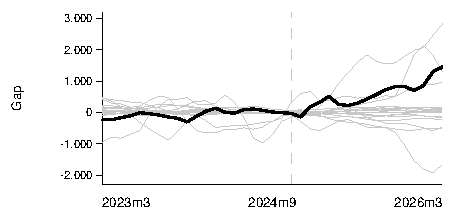
\includegraphics[width=0.486\textwidth]{figures/fig_app-rs_02_emprego_estoque_placebo.pdf}}
\end{minipage}%
}
\caption{Controle sintético, pool Rio Grande do Sul. Painéis à esquerda reportam famílias beneficiárias. Painéis à direita reportam estoque de vínculos formais. Séries em média móvel de 3 meses. No último mês, o efeito é -312 famílias no Bolsa Família ($p_{FP}=0.077$) e 559 vínculos no estoque formal ($p_{FP}=0.095$). Robustez para o pool restrito ao RS.}
\label{fig:app-rs-att}

\end{figure*}


\end{document}
